% Author: Izaak Neutelings (September 2020)
% Inspiration: https://tex.stackexchange.com/questions/25531/adding-underbrace-in-tikz
\documentclass[border=3pt,tikz]{standalone}
\usepackage{physics}
\usepackage{siunitx}
\usepackage{ifthen}
\usepackage{tikz}
\usetikzlibrary{calc}
\usetikzlibrary{angles,quotes} % for pic
\usetikzlibrary{patterns,snakes}
\tikzset{>=latex} % for LaTeX arrow head

\colorlet{xcol}{blue!85!black}
\colorlet{vcol}{green!60!black}
\colorlet{myred}{red!65!black}
\tikzstyle{vvec}=[->,vcol,thick,line cap=round]
\tikzstyle{ground}=[preaction={fill,top color=black!10,bottom color=black!5,shading angle=20},
                    fill,pattern=north east lines,draw=none,minimum width=0.3,minimum height=0.6]
\tikzstyle{metal}=[fill,top color=black!40,bottom color=black!20,shading angle=10]
\tikzstyle{mass}=[line width=0.6,red!30!black,fill=red!40!black!10,rounded corners=1,
                  top color=red!40!black!20,bottom color=red!40!black!10,shading angle=20]
\tikzstyle{pulcol}=[draw=blue!30!black,%fill=blue!40!black!10
                    top color=blue!40!black!20,bottom color=blue!40!black!10,shading angle=20]
\tikzstyle{rope}=[brown!70!black,very thick,line cap=round]
\def\rope#1{ \draw[black,line width=1.5] #1; \draw[rope] #1; }
\tikzstyle{mount}=[blue!20!black,fill,top color=blue!20!black!70,bottom color=blue!20!black!40,shading angle=10] %,line width=1.8,line cap=round
%\tikzstyle{mount}=[color=black!60,line width=1.8,line cap=round]
\tikzstyle{spring}=[line width=0.8,black!80,snake=coil,segment amplitude=5,segment length=5,line cap=round]
\pgfdeclarelayer{back} % to draw on background
\pgfsetlayers{back,main} % set order

% FORCES SWITCH
\tikzstyle{force}=[->,myred,thick,line cap=round]
\newcommand{\vbF}{\vb{F}}
\newcommand{\vbT}{\vb{T}}
\newboolean{showforces}
\setboolean{showforces}{true}

\newcommand\rightAngle[4]{
  \pgfmathanglebetweenpoints{\pgfpointanchor{#2}{center}}{\pgfpointanchor{#3}{center}}
  \coordinate (tmpRA) at ($(#2)+(\pgfmathresult+45:#4)$);
  %\draw[white,line width=0.6] ($(#2)!(tmpRA)!(#1)$) -- (tmpRA) -- ($(#2)!(tmpRA)!(#3)$);
  \draw[blue!40!black] ($(#2)!(tmpRA)!(#1)$) -- (tmpRA) -- ($(#2)!(tmpRA)!(#3)$);
}

% PULLEY
\def\r{0.05} % pulley small radius
\tikzset{
  pics/pulley/.style={
    code={
      \draw[pulcol,line width=0.6] (0,0) circle (#1);
      \draw[pulcol,thick] (0,0) circle (\r);
  }},
  pics/mount/.style args={#1:#2}{ % angle, length
    code={
      \draw[mount] (0,0)++(#1-90:0.9*\r) arc (#1-90:#1-270:0.9*\r) --++ (#1:#2) --++ (#1-90:1.8*\r) -- cycle;
  }},
  pics/weight/.style args={#1,#2,#3}{ % bottom width, top width, height
    code={
      \draw[mass] (0,0) -- (#2/2,0) -- (#1/2,-0.7*#3)
        |- (-#1/2,-#3) -- (-#1/2,-0.7*#3) -- (-#2/2,0) -- cycle;
      \path[mass] (0,0) -- (0,-#3) node[pos=0.52] {$m$};
  }},
  pics/pulley/.default=0.3,
}

\begin{document}


% TABLE + pulley
\def\h{0.6}  % mass height
\def\w{0.8}  % mass width
\def\R{0.3}  % pulley radius
\begin{tikzpicture}
  \def\W{2.2} % ground width
  \def\D{0.3} % ground depth
  \def\L{0.7} % rope length
  \def\p{0.6*\W+\R} % pulley x position
  \draw[ground] (-\W/2,0) rectangle++ (\W,-\D);
  \rope{(0,\h/2) -- (\p,\h/2) arc (90:0:\R) --++ (0,-\L) coordinate (T)}
  \draw (-\W/2,0) --++ (\W,0) --++ (0,-\D);
  \pic at (\p,\h/2-\R) {pulley};
  \draw[mass] (-\w,0) rectangle++ (\w,\h) node[midway] {$m$};
  \draw[mass] (T)++(-\w/2,0) rectangle++ (\w,-\h) node[midway] {$m$};
  
  % FORCES
  \ifthenelse{\boolean{showforces}}{
    \draw[->] (0.48*\W,1.05*\h) --++ (0.7*\w,0) node[right] {$x$};
    \draw[->] (T)++(2.5*\R,0.3*\h) --++ (0,-0.7*\w) node[above=2,right] {$x$};
    \draw[force] (-0.1*\w,0.7*\h) --++ (1.2*\h,0) node[left=3,above=0] {$\vbT_1$};
    \draw[force] (T)++( 0.2*\w,-0.1*\h) --++ (0,1.2*\h) node[below=2,right=0] {$\vbT_2$};
    \draw[force] (T)++(-0.3*\w,-0.6*\h) --++ (0,-1.2*\h) node[below=-3] {$-mg\vu{x}$}; %\vbF_\mathrm{g} = 
  }{}
  
\end{tikzpicture}


% TABLE + pulley spring
\begin{tikzpicture}
  \def\H{0.8} % wall height
  \def\T{0.3} % wall thickness
  \def\W{2.6} % ground length
  \def\D{0.3} % ground depth
  \def\L{0.7}  % rope length
  \def\x{1.4} % mass width
  \def\p{\W+1.8*\R} % pulley x position
  \draw[spring] (0,\h/2) --++ (\x,0);
  \draw[ground] (0,0) -- (0,\H) --++ (-\T,0) --++ (0,-\H-\D) --++
                (\T+\W,0) -- (\W,0) -- cycle;
  \draw (0,\H) -- (0,0) -- (\W,0) --++ (0,-\D);
  \rope{(\x+\h,\h/2) -- (\p,\h/2) arc (90:0:\R) --++ (0,-\L) coordinate (T)}
  \pic at (\p,\h/2-\R) {pulley};
  \draw[mass] (\x,0) rectangle++ (\w,\h) node[midway] {$m$};
  \draw[mass] (T)++(-\w/2,0) rectangle++ (\w,-\h) node[midway] {$m$};
\end{tikzpicture}


% TABLE double
\begin{tikzpicture}
  \def\W{2.4}  % ground width
  \def\D{0.3}  % ground depth
  \def\L{0.7}  % rope length
  \def\pr{0.6*\W+\R} % pulley x position
  \def\pl{-0.6*\W-\R} % pulley x position
  \draw[ground] (-\W/2,0) rectangle++ (\W,-\D);
  \draw (-\W/2,-\D) --++ (0,+\D) --++ (\W,0) --++ (0,-\D);
  \rope{
    (0,\h/2) -- (\pr,\h/2) arc (90:0:\R) --++ (0,-\L) coordinate (TR)
    (0,\h/2) -- (\pl,\h/2) arc (90:180:\R) --++ (0,-\L) coordinate (TL)}
  \pic at (\pl,\h/2-\R) {pulley};
  \pic at (\pr,\h/2-\R) {pulley};
  \draw[mass]
    (-\w/2,0) rectangle++ (\w,\h) node[midway] {$m$}
    (TL)++(-\w/2,0) rectangle++ (\w,-\h) node[midway] {$m$}
    (TR)++(-\w/2,0) rectangle++ (\w,-\h) node[midway] {$m$};
\end{tikzpicture}


% CEILING PULLEY - straight
\begin{tikzpicture}
  \def\W{1.8}  % ground width
  \def\H{2.3}  % ground height
  \def\D{0.3}  % ground depth
  \def\L{0.7}  % rope length
  \def\t{0.1}  % peg thickness
  \def\R{0.30} % pulley radius
  \def\px{0.45*\W} % pulley x position
  \def\py{0.80*\H} % pulley y position
  \def\my{0.30*\H} % mass y position
  \def\rx{\px-1.0*\R} % rope-peg x position
  \coordinate (P) at (\px,\py); % pulley
  \coordinate (M) at (\px+\R,\my); % mass
  \draw[metal,very thin] (0,0.305*\H) rectangle++ (1.07*\rx,\t);
  \rope{ %draw[rope,line cap=round]
    (\rx,0.3*\H) -- (\px-\R,\py) arc(180:0:\R) --++ (0,\my-\py)}
  \pic at (P) {pulley={\R}};
  \pic at (P) {mount={90:\H-\py}};
  \draw[mass] (M)++(-\w/2,0) rectangle++ (\w,-\h) node[midway] {$m$};
  \draw[ground] %(0,0) rectangle++ (-\D,\H) (-\D,\H) rectangle++ (\W,\D);
    (0,0) --++ (0,\H) --++ (\W,0) --++ (0,\D) --++ (-\W-\D,0) -- (-\D,0) -- cycle;
  \draw (0,0) --++ (0,\H) --++ (\W,0);
\end{tikzpicture}


% CEILING PULLEY - slanted
\begin{tikzpicture}
  \def\W{2.0}  % ground width
  \def\H{2.3}  % ground height
  \def\D{0.3}  % ground depth
  \def\L{0.7}  % rope length
  \def\t{0.1}  % peg thickness
  \def\px{0.55*\W} % pulley x position
  \def\py{0.80*\H} % pulley y position
  \def\my{0.30*\H} % mass y position
  \def\rx{\px-2.2*\R} % rope-peg x position
  \coordinate (P) at (\px,\py); % pulley
  \coordinate (M) at (\px+\R,\my); % mass
  \draw[metal,very thin] (0,0.305*\H) rectangle++ (1.07*\rx,\t);
  \rope{ %[rope,line cap=round]
    (\rx,0.3*\H) -- ({\px-\R*cos(19)},{\py+\R*sin(19)}) arc(161:0:\R) --++ (0,\my-\py)}
  \pic at (P) {pulley};
  \pic at (P) {mount={90:\H-\py}};
  \draw[mass] (M)++(-\w/2,0) rectangle++ (\w,-\h) node[midway] {$m$};
  \draw[ground] %(0,0) rectangle++ (-\D,\H) (-\D,\H) rectangle++ (\W,\D);
    (0,0) --++ (0,\H) --++ (\W,0) --++ (0,\D) --++ (-\W-\D,0) -- (-\D,0) -- cycle;
  \draw (0,0) --++ (0,\H) --++ (\W,0);
\end{tikzpicture}


% CEILING PULLEY + ROPE
\begin{tikzpicture}
  \def\W{2.0}  % ceiling width
  \def\H{2.5}  % ceiling height
  \def\D{0.3}  % ceiling depth
  \def\L{0.7}  % rope length
  \def\h{0.6}  % mass height
  \def\w{0.9}  % mass width
  \def\t{0.1}  % peg thickness
  \def\px{0.40*\W} % pulley x position
  \def\py{0.80*\H} % pulley y position
  \def\mx{0.70*\W} % mass x position
  \def\my{0.30*\H} % mass y position
  \coordinate (P) at (\px,\py); % pulley
  \coordinate (M) at (\mx,\my); % mass
  \draw[metal,very thin] (0,0.403*\H) rectangle++ (\px-0.9*\R,\t);
  \rope{ %[rope,line cap=round]
    (\px-\R,0.4*\H) -- (\px-\R,\py) arc(180:0:\R) --++ (0,\my-\py)
    (\mx+0.32*\w,\H) --++ (0,\my-\H)}
  \pic at (P) {pulley};
  \pic at (P) {mount={90:\H-\py}};
  \draw[mass] (M)++(-\w/2,0) rectangle++ (\w,-\h) node[midway] {$m$};
  \draw[ground] %(0,0) rectangle++ (-\D,\H) (-\D,\H) rectangle++ (\W,\D);
    (0,0) --++ (0,\H) --++ (\W,0) --++ (0,\D) --++ (-\W-\D,0) -- (-\D,0) -- cycle;
  \draw (0,0) --++ (0,\H) --++ (\W,0);
\end{tikzpicture}
 

% CEILING PULLEY 3
\begin{tikzpicture}
  \def\W{2.0}  % ceiling width
  \def\H{2.8}  % ceiling height
  \def\D{0.3}  % ceiling depth
  \def\L{0.7}  % rope length
  \def\h{0.6}  % mass height
  \def\w{0.9}  % mass width
  \def\t{0.1}  % peg thickness
  \def\px{0.40*\W}  % pulley x position
  \def\py{0.80*\H}  % pulley y position
  \def\mx{\px+2*\R} % mass x position
  \def\my{0.25*\H}  % mass y position
  \def\Mh{\my+1.3*\R} % pulley mount height
  \coordinate (P)  at (\px,\py); % pulley
  \coordinate (PM) at (\mx,\Mh); % pulley on mass
  \coordinate (M)  at (\mx,\my); % mass
  \draw[metal,very thin] (0,0.403*\H) rectangle++ (\px-0.9*\R,\t);
  \rope{ %[rope,line cap=round]
    (\px-\R,0.4*\H) -- (\px-\R,\py) arc(180:0:\R) -- (\mx-\R,\Mh)
    arc(-180:0:\R) -- (\mx+\R,\H)}
  \pic at (P) {pulley};
  \pic at (P) {mount={90:\H-\py}};
  \pic at (PM) {pulley};
  \pic at (PM) {mount={-90:1.3*\R}};
  \draw[mass] (M)++(-\w/2,0) rectangle++ (\w,-\h) node[midway] {$m$};
  \draw[ground] %(0,0) rectangle++ (-\D,\H) (-\D,\H) rectangle++ (\W,\D);
    (0,0) --++ (0,\H) --++ (\W,0) --++ (0,\D) --++ (-\W-\D,0) -- (-\D,0) -- cycle;
  \draw (0,0) --++ (0,\H) --++ (\W,0);
\end{tikzpicture}


% CEILING PULLEY - person
\begin{tikzpicture}
  \def\W{2.8}  % ground width
  \def\H{2.3}  % ground height
  \def\D{0.3}  % ground depth
  \def\h{0.50} % mass height
  \def\w{0.75} % mass width
  \def\L{0.7}  % rope length
  \def\t{0.1}  % peg thickness
  \def\R{0.30} % pulley radius
  \def\F{0.8}  % force magnitude
  \def\v{0.40} % velocity magnitude
  \def\ang{-100}      % pull angle
  \def\px{0.58*\W}    % pulley x position
  \def\py{0.80*\H}    % pulley y position
  \def\my{0.30*\H}    % mass y position
  \def\rx{\px-1.0*\R} % rope-peg x position
  \def\Hh{2.4}        % human height
  \def\Hw{0.8}        % human width
  \def\Hy{-0.4*\H}    % human y position
  \def\Hx{0.21*\W}    % human x position
  \coordinate (P)  at (\px,\py);    % pulley
  \coordinate (M)  at (\px+\R,\my); % mass
  \coordinate (T)  at ({\px+\R*sin(\ang)},{\py-\R*cos(\ang)}); % mass
  \coordinate (RH) at ($(T)+(\ang:1.3)$); % right hand
  
  % PULLEY & MASS
  \rope{ %draw[rope,line cap=round]
    (RH) -- (T) arc(\ang+270:0:\R) --++ (0,\my-\py)}
  \pic at (P) {pulley={\R}};
  \pic at (P) {mount={90:\H-\py}};
  %\pic at (M) {weight={\w,0.5*\w,\h}};
  \draw[mass] (M)++(-\w/2,0) rectangle++ (\w,-\h) node[midway] {$m$};
  \draw[ground] (0,\H) rectangle++ (\W,\D);
  \draw (0,\H) --++ (\W,0);
  
  % PERSON
  \draw[thick] (\Hx,\Hy+\Hh) circle (0.4) coordinate (H); % head
  \draw[thick,line cap=round] % body
    (H)++(-117:0.4) coordinate (N) to[out=-100,in=110]++ (0,-0.40*\Hh) coordinate (B);
  \begin{pgfonlayer}{back} % draw on back
    \draw[thick,line cap=round] % left arm
      (N)++(-85:0.03) to[out=-70,in=230,looseness=1.2] ($(RH)!0.18!(T)+(0.03,0)$);
  \end{pgfonlayer}
  \draw[thick,line cap=round] % right arm
    (N)++(-85:0.03) to[out=-105,in=220,looseness=1.25] ($(RH)!0.02!(T)+(0.03,0.02)$);
  \draw[thick] (B) to[out=-65,in=72] (\Hx+0.04*\Hw,\Hy); % left leg
  \draw[thick] (B) to[out=-55,in=95] (\Hx+0.39*\Hw,\Hy); % right leg
  
  % FORCES
  \draw[vvec] (M)++(0.7*\w,-0.3*\h) --++ (0,\v) node[above=2,right=-2] {$v$};
  \ifthenelse{\boolean{showforces}}{
    \draw[vvec] (T)++(\ang-16:0.4) --++ (\ang:\v) node[anchor=65,inner sep=1] {$v$};
    \draw[force] (RH)++(\ang+165:0.6*\F) --++ (\ang:\F) node[below=-2] {$\vbT$}; % hand
    \draw[force] (M)++(0.2*\w,0.3*\h) --++ (0,\F) node[right=-2] {$\vbT$};
    \draw[force] (M)++(-0.3*\w,-0.8*\h) --++ (0,-\F) node[below=-3] {$-mg\vu{y}$};
  }{}
  
\end{tikzpicture}
 

% BLOCK & TACKLE with snatch block & person
% https://en.wikipedia.org/wiki/Block_and_tackle
% https://www.youtube.com/watch?v=M2w3NZzPwOM
\begin{tikzpicture}
  \def\W{3.0}  % ceiling width
  \def\H{2.6}  % ceiling height
  \def\D{0.3}  % ceiling depth
  \def\h{0.50} % mass height
  \def\w{0.75} % mass width
  \def\L{0.7}  % rope length
  \def\t{0.08} % peg thickness
  \def\F{0.45} % force magnitude
  \def\v{0.35} % velocity magnitude
  \def\ang{-97}       % pull angle
  \def\R{0.27}        % pulley radius
  \def\px{0.55*\W}    % pulley x position
  \def\py{0.8*\H}     % pulley y position
  \def\mx{\px+2*\R}   % mass x position
  \def\my{0.25*\H}    % mass y position
  \def\Mh{\my+1.3*\R} % pulley mount height
  \def\Hh{2.6}        % human height
  \def\Hw{0.8}        % human width
  \def\Hy{-0.3*\H}    % human y position
  \def\Hx{ 0.19*\W}   % human x position
  \coordinate (P)  at (\px,\py); % pulley
  \coordinate (PM) at (\mx,\Mh); % pulley on mass
  \coordinate (M)  at (\mx,\my); % mass
  \coordinate (T)  at ({\px+\R*sin(\ang)},{\py-\R*cos(\ang)}); % mass
  \coordinate (RH) at ($(T)+(\ang:1.45)$); % right hand
  
  % PULLEY & MASS
  \rope{ %[rope,line cap=round]
    (RH) -- (T) arc(\ang+270:0:\R) -- (\mx-\R,\Mh)
    arc(-180:0:\R) -- (\mx+\R,\H)}
  \pic at (P) {pulley={\R}};
  \pic at (P) {mount={90:\H-\py}};
  \pic at (PM) {pulley={\R}};
  \pic at (PM) {mount={-90:1.3*\R}};
  %\pic at (M) {weight={\w,0.5*\w,\h}};
  \draw[mass] (M)++(-\w/2,0) rectangle++ (\w,-\h) node[midway] {$m$};
  \draw[ground] (0,\H) rectangle++ (\W,\D);
  \draw (0,\H) --++ (\W,0);
  
  % PERSON
  \draw[thick] (\Hx,\Hy+\Hh) circle (0.4) coordinate (H); % head
  \draw[thick] % body
    (H)++(0,-0.4) coordinate (N) to[out=-95,in=95]++ (0,-0.40*\Hh) coordinate (B);
  \begin{pgfonlayer}{back} % draw in back
    \draw[thick,line cap=round] % left arm
      (N)++(-85:0.03) to[out=-70,in=190,looseness=1.1] ($(RH)!0.1!(T)+(0.03,0)$);
  \end{pgfonlayer}
  \draw[thick,line cap=round] % right arm
    (N)++(-85:0.03) to[out=-100,in=190,looseness=1.2] ($(RH)!0.02!(T)+(0.03,0.02)$);
  \draw[thick] (B) to[out=-85,in=82] (\Hx-0.03*\Hw,\Hy); % left leg
  \draw[thick] (B) to[out=-80,in=85] (\Hx+0.15*\Hw,\Hy); % right leg
  
  % FORCES
  \draw[vvec] (M)++(0.7*\w,-0.4*\h) --++ (0,\v) node[above=2,right=-2] {$v$};
  \ifthenelse{\boolean{showforces}}{
    \draw[vvec] (T)++(\ang-40:0.2) --++ (\ang:2*\v) node[anchor=40,inner sep=-1] {$2v$};
    \draw[force] (RH)++(\ang+153:0.5*\F) --++ (\ang:\F) node[below=-2] {$\vbT$}; % hand
    \draw[force] (\mx-1.4*\R,\Mh) --++ (0,\F) node[left=-2] {$\vbT$};  % mass pulley left
    \draw[force] (\mx+1.4*\R,\Mh) --++ (0,\F) node[right=-2] {$\vbT$}; % mass pulley right
    \draw[force] (\mx+1.4*\R,0.98*\H) --++ (0,-\F) node[pos=0.6,right=-1] {$\vbT$}; % hand
    \draw[force] (M)++(-0.3*\w,-0.8*\h) --++ (0,-2*\F) node[below=-3] {$-mg\vu{y}$};
  }{}
  
\end{tikzpicture}


% CEILING PULLEY - two masses
\begin{tikzpicture}
  \def\W{3.7}  % ceiling width
  \def\H{2.4}  % ceiling height
  \def\D{0.3}  % ceiling depth
  \def\px{0.25*\W} % pulley x position
  \def\py{0.80*\H} % pulley y position
  \def\mx{\px+\R}  % mass x position
  \def\my{0.30*\H} % mass y position
  \coordinate (PL) at (-\px,\py); % pulley
  \coordinate (PR) at ( \px,\py); % pulley
  \coordinate (ML) at ({-(\mx)},\my); % mass
  \coordinate (MR) at ( \mx,\my);     % mass
  \rope{ %[rope]
    (ML) -- (-\px-\R,\py) arc (180:90:\R) -- (\px,\py+\R) arc (90:0:\R) -- (MR)}
  \pic at (PL) {pulley};
  \pic at (PR) {pulley};
  \pic at (PR) {mount={90:\H-\py}};
  \pic at (PL) {mount={90:\H-\py}};
  \draw[mass] (ML)++(-\w/2,-\h/2) rectangle++ (\w,\h) node[midway] {$m$};
  \draw[mass] (MR)++(-\w/2,-\h/2) rectangle++ (\w,\h) node[midway] {$m$};
  \draw[ground] (-\W/2,\H) rectangle++ (\W,\D);
  \draw (-\W/2,\H) --++ (\W,0);
  
  % FORCES
  \ifthenelse{\boolean{showforces}}{
    %\draw[->] (ML)++(-1.0*\w,-0.5*\h) --++ (0.7*\w,0) node[right] {$y$};
    %\draw[->] (T)++(2.5*\R,0.3*\h) --++ (0,-0.7*\w) node[above=2,right] {$x$};
    %\draw[force] (-0.1*\w,0.7*\h) --++ (1.2*\h,0) node[left=3,above=0] {$\vbT_1$};
    \draw[force] (ML)++(-0.2*\w, 0.4*\h) --++ (0, 1.2*\h) node[below=2,left=0] {$\vbT_1$};
    \draw[force] (MR)++( 0.2*\w, 0.4*\h) --++ (0, 1.2*\h) node[below=2,right=0] {$\vbT_2$};
    \draw[force] (ML)++(-0.3*\w,-0.1*\h) --++ (0,-1.2*\h) node[below=-3] {$-mg\vu{y}$}; %\vbF_\mathrm{g} = 
    \draw[force] (MR)++(-0.3*\w,-0.1*\h) --++ (0,-1.2*\h) node[below=-3] {$-mg\vu{y}$};
  }{}
  
\end{tikzpicture}


% CEILING PULLEY - three masses with joint
\def\W{4.9}      % ceiling width
\def\H{1.6}      % ceiling height
\def\D{0.3}      % ceiling depth
\def\R{0.30}     % pulley radius
\def\px{0.31*\W} % pulley x position
\def\py{0.80*\H} % pulley y position
\def\mx{\px+\R}  % mass x position
\def\my{0.28*\H} % mass y position
\begin{tikzpicture}
  \def\h{0.53}   % mass height
  \def\ang{48}   % rope angle
  \coordinate (PL) at (-\px,\py); % pulley
  \coordinate (PR) at ( \px,\py); % pulley
  \coordinate (ML) at ({-(\mx)},\my); % mass
  \coordinate (MR) at ( \mx,\my);     % mass
  \coordinate (X)  at (0,1.1*\my);    % rope joint
  \coordinate (M)  at (0,0);          % mass
  \draw[ground] (-\W/2,\H) rectangle++ (\W,\D);
  \draw (-\W/2,\H) --++ (\W,0);
  \rope{ %[rope]
     (ML) -- (-\px-\R,\py) arc (180:\ang:\R)
     -- (X) -- ({\px-\R*cos(\ang)},{\py+\R*sin(\ang)}) arc (180-\ang:0:\R) -- (MR)
     (X) -- (M)}
  \pic at (PL) {pulley};
  \pic at (PR) {pulley};
  \pic at (PR) {mount={90:\H-\py}};
  \pic at (PL) {mount={90:\H-\py}};
  \pic at (ML) {weight={\w,0.5*\w,\h}};
  \pic at (MR) {weight={\w,0.5*\w,\h}};
  \pic at (M)  {weight={\w,0.5*\w,\h}};
  %\draw[mass] (ML)++(-\w/2,-\h/2) rectangle++ (\w,\h) node[midway] {$m$};
  %\draw[mass] (MR)++(-\w/2,-\h/2) rectangle++ (\w,\h) node[midway] {$m$};
  %\draw[mass] (M)++(-\w/2,0) rectangle++ (\w,-\h) node[midway] {$m$};
\end{tikzpicture}


% CEILING PULLEY - three masses without joint
\begin{tikzpicture}
  \def\h{0.53} % mass height
  \def\ang{42} % rope angle
  \coordinate (PL) at (-\px,\py); % pulley
  \coordinate (PR) at ( \px,\py); % pulley
  \coordinate (ML) at ({-(\mx)},\my); % mass
  \coordinate (MR) at ( \mx,\my);     % mass
  \coordinate (M)  at (0,0);          % mass
  \draw[ground] (-\W/2,\H) rectangle++ (\W,\D);
  \draw (-\W/2,\H) --++ (\W,0);
  \rope{ %[rope]
     (ML) -- (-\px-\R,\py) arc (180:\ang:\R)
     -- (M) -- ({\px-\R*cos(\ang)},{\py+\R*sin(\ang)}) arc (180-\ang:0:\R) -- (MR)}
  \pic at (PL) {pulley};
  \pic at (PR) {pulley};
  \pic at (PR) {mount={90:\H-\py}};
  \pic at (PL) {mount={90:\H-\py}};
  \pic at (ML) {weight={\w,0.5*\w,\h}};
  \pic at (MR) {weight={\w,0.5*\w,\h}};
  \pic at (M)  {weight={\w,0.5*\w,\h}};
  %\draw[mass] (ML)++(-\w/2,-\h/2) rectangle++ (\w,\h) node[midway] {$m$};
  %\draw[mass] (MR)++(-\w/2,-\h/2) rectangle++ (\w,\h) node[midway] {$m$};
  %\draw[mass] (M)++(-\w/2,0) rectangle++ (\w,-\h) node[midway] {$m$};
\end{tikzpicture}


% CEILING PULLEY - three unequal masses
\begin{tikzpicture}
  \def\W{4.9}  % ceiling width
  \def\H{2.5}  % ceiling height
  \def\D{0.3}  % ceiling depth
  \def\px{0.31*\W} % pulley x position
  \def\py{0.80*\H} % pulley y position
  \def\mx{\px+\R}  % mass x position
  \def\my{0.20*\H} % mass y position
  \coordinate (PL) at (-\px,\py); % pulley
  \coordinate (PR) at ( \px,\py); % pulley
  \coordinate (ML) at ({-(\mx)},0.7*\my); % mass
  \coordinate (MR) at ( \mx,1.2*\my);     % mass
  \coordinate (X)  at (-0.1*\W,0.40*\H);  % mass
  \coordinate (M)  at (-0.1*\W,0.15*\H);  % mass
  \draw[ground] (-\W/2,\H) rectangle++ (\W,\D);
  \draw (-\W/2,\H) --++ (\W,0);
  \rope{ %[rope]
     (ML) -- (-\px-\R,\py) arc (180:35:\R) coordinate (PLT)
     -- (X) -- ({\px-\R*cos(55)},{\py+\R*sin(55)}) coordinate (PRT) arc (125:0:\R) -- (MR)
     (X) -- (M)}
  \pic at (PL) {pulley};
  \pic at (PR) {pulley};
  \pic at (PR) {mount={90:\H-\py}};
  \pic at (PL) {mount={90:\H-\py}};
  \draw[mass] (ML)++(-\w/2,-\h/2) rectangle++ (\w,\h) node[midway] {\;$m_1$};
  \draw[mass] (MR)++(-\w/2,-\h/2) rectangle++ (\w,\h) node[midway] {\;$m_3$};
  \draw[mass] (M)++(-\w/2,0) rectangle++ (\w,-\h) node[midway] {\;$m_2$};
  %\rightAngle{PLT}{X}{PRT}{0.4}
  \draw[dashed] (X) --++ (0,0.3*\H) coordinate (T);
  \draw pic["$\theta_1$",xcol,draw=xcol,angle radius=14,angle eccentricity=1.45] {angle=T--X--PLT};
  \draw pic["$\theta_3$",xcol,draw=xcol,angle radius=13,angle eccentricity=1.40] {angle=PRT--X--T};
  
  % FORCES
  \ifthenelse{\boolean{showforces}}{
    \draw[force] (ML)++(-0.2*\w, 0.4*\h) --++ (0, 1.2*\h) node[below=2,left=0] {$\vbT_1$};
    \draw[force] (M)++( -0.2*\w,-0.1*\h) --++ (0, 1.2*\h) node[below=2,left=0] {$\vbT_2$};
    \draw[force] (MR)++(-0.2*\w, 0.4*\h) --++ (0, 1.2*\h) node[below=2,left=0] {$\vbT_3$};
    \draw[force] (ML)++(-0.3*\w,-0.1*\h) --++ (0,-1.2*\h) node[below=-3] {$-m_1g\vu{y}$};
    \draw[force] (M)++( -0.3*\w,-0.6*\h) --++ (0,-1.2*\h) node[below=-3] {$-m_2g\vu{y}$};
    \draw[force] (MR)++(-0.3*\w,-0.1*\h) --++ (0,-1.2*\h) node[below=-3] {$-m_3g\vu{y}$};
    \draw[very thin,metal] (X) circle (0.05);
  }{}
  
\end{tikzpicture}


% CEILING PULLEY - three unequal masses - forces
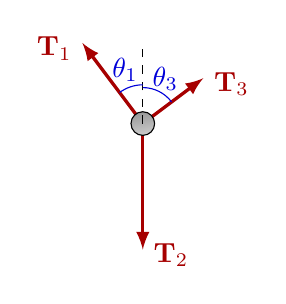
\begin{tikzpicture}
  \def\F{1.6}
  \coordinate (O) at (0,0);
  \draw[force,very thick] (O) -- ({acos(4/5)+90}:4/5*\F) coordinate (F1) node[below=2,left=0] {$\vbT_1$};
  \draw[force,very thick] (O) -- ({acos(4/5)}:3/5*\F) coordinate (F3) node[below=2,right=0] {$\vbT_3$};
  \draw[force,very thick] (O) -- (-90:\F) node[below=2,right=0] {$\vbT_2$};
  \draw[thin,metal] (O) circle (0.15);
  %\rightAngle{F1}{O}{F3}{0.4}
  \draw[dashed] (O) --++ (0,0.6*\F) coordinate (T);
  \draw pic["$\theta_1$",xcol,draw=xcol,angle radius=14,angle eccentricity=1.45] {angle=T--O--F1};
  \draw pic["$\theta_3$",xcol,draw=xcol,angle radius=13,angle eccentricity=1.40] {angle=F3--O--T};
\end{tikzpicture}


% CEILING PULLEY - three unequal masses - forces triangle
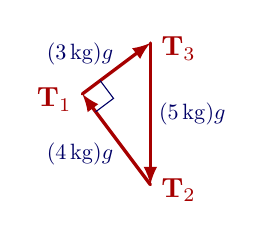
\begin{tikzpicture}
  \def\F{1.8}
  \coordinate (O) at (0,0);
  \draw[force,very thick] (O) -- ({acos(4/5)+90}:4/5*\F) coordinate (F1)
    node[blue!40!black,midway,below left=-2,scale=0.8] {$(\SI{4}{kg})g$} node[below=2,left=0] {$\vbT_1$};
  \draw[force,very thick] (F1) -- (90:\F) coordinate (F3)
    node[blue!40!black,midway,above left=-2,scale=0.8] {$(\SI{3}{kg})g$} node[below=2,right=0] {$\vbT_3$};
  \draw[force,very thick] (F3) -- (O)
    node[blue!40!black,midway,right=0,scale=0.8] {$(\SI{5}{kg})g$} node[below=2,right=0] {$\vbT_2$};
  \rightAngle{F3}{F1}{O}{0.4}
\end{tikzpicture}


\end{document}